\caulc
\begin{ex}%[2D4N1-3] %[TDMZZ27]%[ Trần Văn Thiện, Nguyễn Sơn Thành]
	Nguyên hàm của hàm số $y = \dfrac{1}{\sin^2 x}$ là
	\choice
	{\True $-\cot x + C$}
	{$\cot x + C$}
	{$-\cos x + C$}
	{$-\dfrac{1}{\sin x} + C$}
	\loigiai{
		Ta có $\displaystyle\int \dfrac{1}{\sin^2 x} \mathrm{\,d}x = -\cot x + C$.
	}
\end{ex}

\begin{ex}%[2D4H3-3]%[TDMZZ27]%[ Trần Văn Thiện, Nguyễn Sơn Thành]
	Cho hình phẳng $(H)$ giới hạn bởi các đường $y = 6x - x^2$, $y = 0$. Hãy tính thể tích khối tròn xoay thu được khi cho $(H)$ quay quanh trục hoành $Ox$.
	\choice
	{\True $\dfrac{1\,296\pi}{5}$}
	{$36$}
	{$\dfrac{1\,296}{5}$}
	{$36\pi$}
	\loigiai{
		Phương trình hoành độ giao điểm của hai đường $y = 6x - x^2$ và $y = 0$ là
		\[ 6x - x^2 = 0 \Leftrightarrow \hoac{&x=0 \\ &x=6.} \]
		Thể tích khối tròn xoay thu được là
		\[ V = \pi \displaystyle\int\limits_0^6 \left(6x - x^2\right)^2 \mathrm{\,d}x = \pi \displaystyle\int\limits_0^6 \left(36x^2 - 12x^3 + x^4\right) \mathrm{\,d}x = \pi \left.\left( 12x^3 - 3x^4 + \dfrac{x^5}{5} \right)\right|_0^6 = \dfrac{1\,296\pi}{5}. \]
	}
\end{ex}

\begin{ex}%[2D3H2-3] %[TDMZZ27]%[ Trần Văn Thiện, Nguyễn Sơn Thành]
	Cho hai mẫu số liệu ghép nhóm $M_1$, $M_2$ với bảng tần số ghép nhóm:
	\begin{center}
		\begin{tabular}{|c|c|c|c|c|c|c|c|}
			\hline
			\multirow{2}{*}{$M_1$} & Nhóm & $[2;3)$ & $[3;4)$ & $[4;5)$ & $[5;6)$ & $[6;7)$ & $[7;8)$ \\
			\cline{2-8}
			& Tần số & $5$ & $4$ & $6$ & $4$ & $2$ & $4$ \\
			\hline
		\end{tabular}
		
		\vspace{0.2cm}
		\begin{tabular}{|c|c|c|c|c|c|c|c|}
			\hline
			\multirow{2}{*}{$M_2$} & Nhóm & $[2;3)$ & $[3;4)$ & $[4;5)$ & $[5;6)$ & $[6;7)$ & $[7;8)$ \\
			\cline{2-8}
			& Tần số & $10$ & $8$ & $12$ & $8$ & $4$ & $8$ \\
			\hline
		\end{tabular}
	\end{center}
	Gọi $s_1$, $s_2$ lần lượt là độ lệch chuẩn của hai mẫu số liệu $M_1$, $M_2$. Đáp án so sánh đúng là
	\choice
	{$s_1 > s_2$}
	{\True $s_1 = s_2$}
	{$s_1 = 2s_2$}
	{$s_1 < s_2$}
	\loigiai{
		Gọi $f_{1i}$ là tần số của nhóm thứ $i$ trong mẫu $M_1$ ($i=1,2,\dots,6$).\\
		Tổng số liệu mẫu $M_1$ là $n_1 = 25$.\\
		Gọi $f_{2i}$ là tần số của nhóm thứ $i$ trong mẫu $M_2$.\\ Tổng số liệu mẫu $M_2$ là $n_2 = 50$.\\
		Từ bảng thống kê ta thấy $n_2 = 2n_1$, $f_{2i} = 2f_{1i}$ với mọi $i$.\\
		Giá trị đại diện của nhóm thứ $i$ (gọi là $c_i$) trong hai mẫu là như nhau.\\
		Số trung bình của mẫu $M_1$ là $\overline{x}_1 = \dfrac{1}{n_1}\displaystyle\sum\limits_{i=1}^6 f_{1i} c_i$.\\
		Số trung bình của mẫu $M_2$ là $\overline{x}_2 = \dfrac{1}{n_2}\displaystyle\sum\limits_{i=1}^6 f_{2i} c_i = \dfrac{1}{2n_1}\displaystyle\sum\limits_{i=1}^6 2f_{1i} c_i = \dfrac{1}{n_1}\displaystyle\sum\limits_{i=1}^6 f_{1i} c_i = \overline{x}_1$.\\
		Phương sai của mẫu $M_1$ là $s_1^2 = \dfrac{1}{n_1}\displaystyle\sum\limits_{i=1}^6 f_{1i} (c_i - \overline{x}_1)^2$.\\
		Phương sai của mẫu $M_2$ là $s_2^2 = \dfrac{1}{n_2}\displaystyle\sum\limits_{i=1}^6 f_{2i} (c_i - \overline{x}_2)^2 = \dfrac{1}{2n_1}\displaystyle\sum\limits_{i=1}^6 2f_{1i} (c_i - \overline{x}_1)^2 = s_1^2$.\\
		Vì $s_1^2 = s_2^2$ nên $s_1 = s_2$.
	}
\end{ex}

\begin{ex}%[2H5N1-3] %[TDMZZ27]%[ Trần Văn Thiện, Nguyễn Sơn Thành]
	Trong không gian $Oxyz$, phương trình tổng quát của mặt phẳng $(\alpha)$ có vectơ pháp tuyến $\overrightarrow{n} = (2; 2; -1)$ và đi qua điểm $A(2; 1; 0)$ là
	\choice
	{$(\alpha) \colon 2x + 2y - z + 6 = 0$}
	{$(\alpha) \colon 2x + y - 5 = 0$}
	{$(\alpha) \colon 2x + 2y - z - 3 = 0$}
	{\True $(\alpha) \colon 2x + 2y - z - 6 = 0$}
	\loigiai{
		Mặt phẳng $(\alpha)$ đi qua điểm $A(2; 1; 0)$ và có một vectơ pháp tuyến $\overrightarrow{n} = (2; 2; -1)$ nên có phương trình tổng quát là
		\[ 2(x - 2) + 2(y - 1) - 1(z - 0) = 0 \Leftrightarrow 2x + 2y - z - 6 = 0. \]
	}
\end{ex}

\begin{ex}%[1H8H1-2] % [TDMZZ27]%[Trần Văn Thiện, Nguyễn Sơn Thành]
	\immini{
		Cho hình lập phương $ABCD.A'B'C'D'$. Hỏi cặp đường thẳng nào dưới đây \textbf{không} vuông góc với nhau?
		\choice
		{\True $AB$, $C'D'$}
		{$AC$, $B'D'$}
		{$AB'$, $CD'$}
		{$AC$, $BD'$}
	}{
		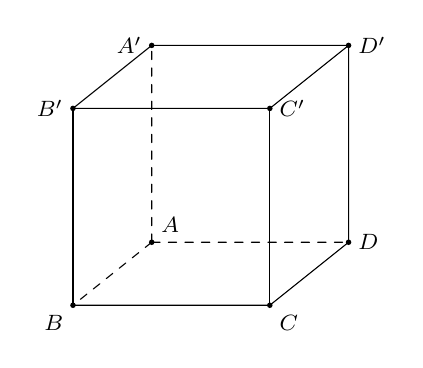
\begin{tikzpicture}[scale=1, font=\footnotesize, line join=round, line cap=round, >=stealth]
			\def\a{2.5}
			\def\x{1}
			\def\y{0.8}
			\coordinate (B) at (0,0);
			\coordinate (C) at (\a,0);
			\coordinate (A) at (\x,\y);
			\coordinate (D) at (\a+\x,\y);
			\coordinate (B') at (0,\a);
			\coordinate (C') at (\a,\a);
			\coordinate (A') at (\x,\a+\y);
			\coordinate (D') at (\a+\x,\a+\y);
			\draw (B) -- (C) -- (D) -- (D') -- (C') -- (B') -- cycle;
			\draw (C) -- (C');
			\draw (B') -- (B) ;
			\draw (A') -- (B') (A') -- (D');
			\draw[dashed] (A) -- (B) (A) -- (D) (A) -- (A');
			\fill (A) circle (1pt) node[above right] {$A$};
			\fill (B) circle (1pt) node[below left] {$B$};
			\fill (C) circle (1pt) node[below right] {$C$};
			\fill (D) circle (1pt) node[right] {$D$};
			\fill (A') circle (1pt) node[left] {$A'$};
			\fill (B') circle (1pt) node[left] {$B'$};
			\fill (C') circle (1pt) node[right] {$C'$};
			\fill (D') circle (1pt) node[right] {$D'$};
		\end{tikzpicture}
	}
	\loigiai{
		Ta có $ABCD.A'B'C'D'$ là hình lập phương nên $AB \parallel CD$ và $CD \parallel C'D'$. Suy ra $AB \parallel C'D'$.\\
		Do đó hai đường thẳng $AB$ và $C'D'$ song song (không vuông góc với nhau).
		\begin{itemize}
			\item Xét đáp án $AC$, $B'D'$: Ta có $AC \perp BD$ (tính chất hình vuông) và $BD \parallel B'D'$ nên $AC \perp B'D'$.
			\item Xét đáp án $AB'$, $CD'$: Ta có $AB' \parallel DC'$ và $DC' \perp CD'$ (hai đường chéo của hình vuông $CDD'C'$) nên $AB' \perp CD'$.
			\item Xét đáp án $AC$, $BD'$: Ta có $AC \perp BD$ và $AC \perp DD' \Rightarrow AC \perp (BDD'B') \Rightarrow AC \perp BD'$.
		\end{itemize}
	}
\end{ex}

\begin{ex}%[2D1H4-1]%[TDMZZ27]%[Trần Văn Thiện, Nguyễn Sơn Thành]
	Tổng số đường tiệm cận đứng và tiệm cận ngang của đồ thị hàm số $y = \dfrac{x^2+2x+1}{x-1}$ là
	\choice
	{\True $1$}
	{$2$}
	{$3$}
	{$0$}
	\loigiai{
		Tập xác định $\mathscr{D} = \mathbb{R} \setminus \{1\}$.\\
		Ta có $\lim\limits_{x \to 1^+} y = \lim\limits_{x \to 1^+} \dfrac{x^2+2x+1}{x-1} = +\infty$ và $\lim\limits_{x \to 1^-} y = -\infty$ nên đường thẳng $x=1$ là tiệm cận đứng của đồ thị hàm số.\\
		Mặt khác $y = \dfrac{x^2+2x+1}{x-1}=x+3+\dfrac{4}{x-1}$.\\
		Khi đó $\lim\limits_{x \to \pm\infty} y = \lim\limits_{x \to \pm\infty}\left(x+3+\dfrac{4}{x-1}\right) = \pm\infty$.\\
		Do đó đồ thị hàm số không có đường tiệm cận ngang.\\
		Vậy đồ thị hàm số có đúng $1$ đường tiệm cận (tiệm cận đứng).
	}
\end{ex}

\begin{ex}% [1D6H4-3][TDMZZ27]%[Trần Văn Thiện, Nguyễn Sơn Thành]
	Tập nghiệm của bất phương trình $\ln(2x-4) < \ln(x+1)$ là
	\choice
	{$\{2; 5\}$}
	{\True $(2; 5)$}
	{$(5; +\infty)$}
	{$(-\infty; 5)$}
	\loigiai{
		Điều kiện xác định $\heva{& 2x - 4 > 0 \\ & x + 1 > 0} \Leftrightarrow \heva{& x > 2 \\ & x > -1} \Leftrightarrow x > 2$.\\
		Bất phương trình đã cho tương đương với $2x - 4 < x + 1 \Leftrightarrow x < 5$.\\
		Kết hợp với điều kiện, ta được $2 < x < 5$.\\
		Vậy tập nghiệm của bất phương trình là $(2; 5)$.
	}
\end{ex}

\begin{ex}%[2H5N2-2][TDMZZ27]%[Trần Văn Thiện, Nguyễn Sơn Thành]
	Trong không gian $Oxyz$, cho đường thẳng $\Delta \colon \dfrac{x-1}{3} = \dfrac{y-2}{2} = \dfrac{z+2}{1}$. Hỏi vectơ nào dưới đây là một vectơ chỉ phương của đường thẳng $\Delta$?
	\choice
	{$\overrightarrow{u}_1 = (2; 1; 3)$}
	{$\overrightarrow{u}_2 = (1; 2; -2)$}
	{$\overrightarrow{u}_3 = (2; 1; 2)$}
	{\True $\overrightarrow{u}_4 = (3; 2; 1)$}
	\loigiai{
		Dựa vào phương trình chính tắc của đường thẳng $\Delta$, ta có một vectơ chỉ phương là $\overrightarrow{u} = (3; 2; 1)$.
		Do đó $\overrightarrow{u}_4 = (3; 2; 1)$ là một vectơ chỉ phương của đường thẳng $\Delta$.
	}
\end{ex}

\begin{ex}%[1D6H4-4][TDMZZ27]%[Trần Văn Thiện, Nguyễn Sơn Thành]
	Số nghiệm thực của phương trình $2^{x^2} = 4^{4x-4}$ là
	\choice
	{$0$}
	{$1$}
	{\True $2$}
	{$3$}
	\loigiai{
		Ta có
		\begin{align*}
			2^{x^2} = 4^{4x-4} &\Leftrightarrow 2^{x^2} = \left(2^2\right)^{4x-4} \\
			&\Leftrightarrow 2^{x^2} = 2^{8x-8} \\
			&\Leftrightarrow x^2 = 8x - 8 \\
			&\Leftrightarrow x^2 - 8x + 8 = 0.
		\end{align*}
		Phương trình bậc hai trên có $\Delta' = (-4)^2 - 1 \cdot 8 = 8 > 0$ nên có $2$ nghiệm thực phân biệt.\\
		Vậy phương trình đã cho có $2$ nghiệm thực.
	}
\end{ex}

\begin{ex}%[1D2H2-5]%[TDMZZ27]%[Trần Văn Thiện, Nguyễn Sơn Thành]
	Cho ba số $a, b, c$ theo thứ tự lập thành một cấp số cộng có tổng bằng $15$. Hãy tính giá trị của $b^2 - (a + c)$?
	\choice
	{$-5$}
	{\True $15$}
	{$5$}
	{$10$}
	\loigiai{
		Vì ba số $a, b, c$ theo thứ tự lập thành một cấp số cộng nên ta có $a + c = 2b$.\\
		Theo giả thiết, tổng của chúng bằng $15$ nên
		\[ a + b + c = 15 \Leftrightarrow 2b + b = 15 \Leftrightarrow 3b = 15 \Leftrightarrow b = 5. \]
		Suy ra $a + c = 2 \cdot 5 = 10$.\\
		Vậy $b^2 - (a + c) = 5^2 - 10 = 25 - 10 = 15$.
	}
\end{ex}

\begin{ex}%[2H2H1-3]
	\immini{
		Trong không gian cho hình lập phương $ABCD.A'B'C'D'$. Đáp án nhận xét đúng là
		\choice
		{$\left(\overrightarrow{AC}, \overrightarrow{DB}\right) = 60^\circ$}
		{$\left(\overrightarrow{AC}, \overrightarrow{AA'}\right) = 45^\circ$}
		{$\left(\overrightarrow{AC}, \overrightarrow{AC'}\right) = 45^\circ$}
		{\True $\left(\overrightarrow{AC}, \overrightarrow{D'C}\right) = 60^\circ$}
	}{
		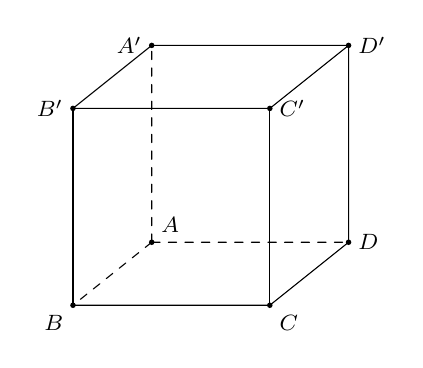
\begin{tikzpicture}[scale=1, font=\footnotesize, line join=round, line cap=round, >=stealth]
			\def\a{2.5}
			\def\x{1}
			\def\y{0.8}
			\coordinate (B) at (0,0);
			\coordinate (C) at (\a,0);
			\coordinate (A) at (\x,\y);
			\coordinate (D) at (\a+\x,\y);
			\coordinate (B') at (0,\a);
			\coordinate (C') at (\a,\a);
			\coordinate (A') at (\x,\a+\y);
			\coordinate (D') at (\a+\x,\a+\y);
			\draw (B) -- (C) -- (D) -- (D') -- (C') -- (B') -- cycle;
			\draw (C) -- (C');
			\draw (B') -- (B) ;
			\draw (A') -- (B') (A') -- (D');
			\draw[dashed] (A) -- (B) (A) -- (D) (A) -- (A');
			\fill (A) circle (1pt) node[above right] {$A$};
			\fill (B) circle (1pt) node[below left] {$B$};
			\fill (C) circle (1pt) node[below right] {$C$};
			\fill (D) circle (1pt) node[right] {$D$};
			\fill (A') circle (1pt) node[left] {$A'$};
			\fill (B') circle (1pt) node[left] {$B'$};
			\fill (C') circle (1pt) node[right] {$C'$};
			\fill (D') circle (1pt) node[right] {$D'$};
		\end{tikzpicture}
	}
	\loigiai{
		Kiểm tra từng phương án:
		\begin{itemize}
			\item Vì $ABCD$ là hình vuông nên $AC \perp BD \Rightarrow \left(\overrightarrow{AC}, \overrightarrow{DB}\right) = 90^\circ$. Phương án $\left(\overrightarrow{AC}, \overrightarrow{DB}\right) = 60^\circ$ sai.
			\item Ta có $AA' \perp (ABCD)$ nên $AA' \perp AC \Rightarrow \left(\overrightarrow{AC}, \overrightarrow{AA'}\right) = 90^\circ$. Phương án $\left(\overrightarrow{AC}, \overrightarrow{AA'}\right) = 45^\circ$ sai.
			\item Xét tam giác vuông $AA'C$, ta có $\cos \widehat{A'CA} = \dfrac{AC}{AC'} = \dfrac{a\sqrt{2}}{a\sqrt{3}} = \dfrac{\sqrt{6}}{3} \neq \cos 45^\circ$.\\ Phương án $\left(\overrightarrow{AC}, \overrightarrow{AC'}\right) = 45^\circ$ sai.
			\item Xét góc giữa hai vectơ $\overrightarrow{AC}$ và $\overrightarrow{D'C}$. Ta có
			\[ \left(\overrightarrow{AC}, \overrightarrow{D'C}\right) = \left(-\overrightarrow{CA}, -\overrightarrow{CD'}\right) = \left(\overrightarrow{CA}, \overrightarrow{CD'}\right) = \widehat{ACD'}. \]
			Lại có $AC = CD' = AD' = a\sqrt{2}$ (vì đều là đường chéo của các mặt hình vuông cạnh $a$).\\
			Suy ra tam giác $ACD'$ là tam giác đều, do đó $\widehat{ACD'} = 60^\circ$. Phương án $\left(\overrightarrow{AC}, \overrightarrow{D'C}\right) = 60^\circ$ đúng.
		\end{itemize}
	}
\end{ex}

\begin{ex}%[2D1H5-7]%[TDMZZ27]%[Trần Văn Thiện, Nguyễn Sơn Thành]
	Đồ thị hàm số $y = \dfrac{x+3}{x-2}$ có tâm đối xứng cách gốc tọa độ một đoạn bằng
	\choice
	{$2$}
	{$1$}
	{\True $\sqrt{5}$}
	{$\sqrt{3}$}
	\loigiai{
		Đồ thị hàm số $y = \dfrac{x+3}{x-2}$ có tiệm cận đứng là đường thẳng $x = 2$; đường tiệm cận ngang là đường thẳng $y = 1$.\\
		Tâm đối xứng $I$ của đồ thị hàm số là giao điểm của hai đường tiệm cận, do đó $I(2; 1)$.\\
		Khoảng cách từ tâm đối xứng $I$ đến gốc tọa độ $O(0; 0)$ là
		\[ OI = \sqrt{2^2 + 1^2} = \sqrt{5}. \]
	}
\end{ex}
\cauds
\begin{ex}%[2D1H5-7]%[Dương Công Tạo]
	Trong mặt phẳng toạ độ $Oxy$, cho hàm số $y = \dfrac{x+5}{x-1}$ có đồ thị $(C)$.
	\choiceTF
	{\True Tập xác định của hàm số là $\mathscr{D} = (-\infty;1)\cup(1;+\infty)$}
	{\True Hàm số nghịch biến trên $(-\infty;1);(1;+\infty)$}
	{\True $(C)$ có tâm đối xứng là $(1;1)$}
	{\True Có $8$ điểm có toạ độ nguyên thuộc $(C)$}
	\loigiai{
		\begin{itemchoice}
			\itemch Tập xác định của hàm số là $\mathscr{D} = (-\infty;1)\cup(1;+\infty)$.
			\itemch Ta có $y'= \dfrac{-6}{(x-1)^2}<0$, $\forall x\neq 1$. Do đó, hàm số nghịch biến trên $(-\infty;1);(1;+\infty)$.
			\itemch Ta có \begin{itemize}
				\item Ta có $\lim\limits_{x\to 1^-}y=-\infty$ suy ra $x=1$ là tiệm cận đứng của $(C)$.
				\item Ta có $\lim\limits_{x\to \pm\infty}y=1$ suy ra $y=1$ là tiệm cận đứng của $(C)$.
			\end{itemize}
			Do đó, đồ thị $(C)$ có tâm đối xứng là $(1;1)$.
			\itemch Với $x\neq 1$, ta có $y = \dfrac{x+5}{x-1}=1+\dfrac{6}{x-1}$.\\
			Gọi $M(x;y)\in(C)$, với $x$, $y\in\mathbb{Z}$ thì $\dfrac{6}{x-1}\in\mathbb{Z}$.\\
			Suy ra $(x-1)\in\text{ Ư}(6)=\left\{\pm6;\pm3;\pm2;\pm 1\right\}$.\\
			Vậy, có $8$ điểm có toạ độ nguyên thuộc $(C)$.
		\end{itemchoice}
	}
\end{ex}

\begin{ex}%[TDMZZ20]%[Hà Văn Hảo]%[2D4V3-1]
	Trên mặt phẳng tọa độ $Oxy$, hình phẳng $(H)$ (được tô màu) giới hạn bởi đường thẳng $x = -6$ và hai đường parabol $y = f(x)$, $y = g(x)$ có các đỉnh nằm trên trục tung $Oy$ như hình vẽ.
	\begin{center}
		\begin{tikzpicture}[>=stealth, scale=0.7]
			\coordinate (B) at (-6,-4);
			\coordinate (C) at (5,-4);
			\coordinate (D) at (5,3);
			\coordinate (A) at (-6,3);
			\coordinate (E) at (-5,0);
			\coordinate (F) at (5,0); 
			\fill[blue!15] plot[domain=-5:5, samples=100] (\x, {-3/25*\x*\x + 3}) -- 
			plot[domain=5:-5, samples=100] (\x, {4/25*\x*\x - 4}) -- cycle;
			
			\fill[blue!15] plot[domain=-6:-5, samples=50] (\x, {-3/25*\x*\x + 3}) -- (-5,0) -- (-6,0) -- cycle;
			\fill[blue!15] plot[domain=-6:-5, samples=50] (\x, {4/25*\x*\x - 4}) -- (-5,0) -- (-6,0) -- cycle;
			
			\path[pattern=north west lines, pattern color=black!80] 
			(-6,3) -- (0,3) 
			-- plot[domain=0:-5, samples=50] (\x, {-3/25*\x*\x + 3}) 
			-- plot[domain=-5:-6, samples=50] (\x, {4/25*\x*\x - 4}) 
			-- cycle; 
			\draw[blue, thick] plot[domain=-6:5.2, samples=100] (\x, {-3/25*\x*\x + 3});
			\draw[blue, thick] plot[domain=-6:5.2, samples=100] (\x, {4/25*\x*\x - 4});
			
			\draw[red, thick] (A) -- (D) -- (C) -- (B) -- cycle;
			\draw[->] (-7,0) -- (6.5,0) node[below] {$x$};
			\draw[->] (0,-5) -- (0,4.5) node[left] {$y$};
			\fill (0,0) circle (2pt) node[below left] {$O$};
			
			\fill (B) circle (1.5pt) node[below] {$B(-6;-4)$};
			\fill (D) circle (1.5pt) node[right] {$D(5;3)$};
			\node[above left] at (A) {$A$};
			\node[below right] at (C) {$C$};
			
			\fill (E) circle (2pt) node[below] {$E$};
			
			\node[above right] at (3.5, 1.3) {$f(x)$};
			\node[below right] at (3.5, -2) {$g(x)$};
			\node at (1, 0.8) {$(H)$};
		\end{tikzpicture}
	\end{center}
	
	\choiceTF
	{\True $f(x) = -\dfrac{3}{25}x^2 + 3$}
	{\True $AE = \sqrt{10}$}
	{Diện tích hình phẳng $(H)$ bằng $\dfrac{1\,124}{25}$}
	{Diện tích phần hình phẳng được gạch chéo trong hình vẽ bằng $12{,}65$ \textit{(làm tròn kết quả đến hàng phần trăm)}}
	\loigiai{
		\begin{itemchoice}
			\itemch Vì parabol $y = f(x)$ có đỉnh nằm trên trục tung $Oy$ nên có dạng $f(x) = ax^2 + c$.\\
			Dựa vào hình vẽ, đỉnh của $f(x)$ là $(0; 3)$ nên $c = 3$.\\
			Đồ thị đi qua điểm $E(-5; 0)$.\\
			Ta có $f(-5) = a \cdot (-5)^2 + 3 = 0 \Leftrightarrow 25a = -3 \Leftrightarrow a = -\dfrac{3}{25}$.\\
			Vậy $f(x) = -\dfrac{3}{25}x^2 + 3$.
			\itemch Ta có $A(-6; 3)$ và $E(-5; 0)$, do đó
			\[AE = \sqrt{(-5 - (-6))^2 + (0 - 3)^2} = \sqrt{1^2 + (-3)^2} = \sqrt{10}.\]
			\itemch Parabol $y = g(x)$ có đỉnh $(0; -4)$ và đi qua điểm $E(-5; 0)$.\\
			Ta có $g(x) = bx^2 - 4 \Rightarrow g(-5) = b \cdot (-5)^2 - 4 = 0 \Leftrightarrow b = \dfrac{4}{25}$.\\
			Suy ra $g(x) = \dfrac{4}{25}x^2 - 4$.\\
			Diện tích hình phẳng $(H)$ giới hạn bởi $x = -6$, $x = 5$, $y = f(x)$ và $y = g(x)$ xác định bởi
			\allowdisplaybreaks
			\begin{eqnarray*}
				S_{(H)} &=& \displaystyle\int\limits_{-6}^{5} \left|f(x) - g(x)\right|\,\mathrm{d}x \\
				&=& \displaystyle\int\limits_{-6}^{5} \left|-\dfrac{3}{25}x^2 + 3 - \left(\dfrac{4}{25}x^2 - 4\right)\right|\,\mathrm{d}x\\
				&=& \displaystyle\int\limits_{-6}^{5} \left|-\dfrac{7}{25}x^2 + 7\right|\,\mathrm{d}x \\
				&=& \dfrac{1\,024}{25}.
			\end{eqnarray*}
			\itemch Phần gạch chéo giới hạn bởi $x = -6$, đường thẳng $y = 3$, parabol $y = f(x)$ và parabol $y = g(x)$.
			\allowdisplaybreaks
			\begin{eqnarray*}
				S_{gc} &=& \displaystyle\int\limits_{-6}^{-5} (3 - g(x))\,\mathrm{d}x + \displaystyle\int\limits_{-5}^{0} (3 - f(x))\,\mathrm{d}x\\
				&=& \displaystyle\int\limits_{-6}^{-5} \left(3 - \left(\dfrac{4}{25}x^2 -4\right)\right)\,\mathrm{d}x + \displaystyle\int\limits_{-5}^{0} \left(3 - \left(-\dfrac{3}{25}x^2 + 3\right)\right)\,\mathrm{d}x \\
				&=& \displaystyle\int\limits_{-6}^{-5} \left(7 - \dfrac{4}{25}x^2\right)\,\mathrm{d}x + \displaystyle\int\limits_{-5}^{0} \dfrac{3}{25}x^2\,\mathrm{d}x\\
				&= & \dfrac{536}{75} \\
				&\approx& 7{,}15.
			\end{eqnarray*}
		\end{itemchoice}
	}
\end{ex}

\begin{ex}%[2D6V2-4]%[TDMZZ27]%[Vũ Hồng Toàn]
	Công ty X có giao cho hai xí nghiệp I và II sản xuất một loại sản phẩm Y. Xí nghiệp I sản xuất $60\%$ tổng sản phẩm với tỉ lệ phế phẩm là $4\%$, xí nghiệp II với tỉ lệ sản phẩm tốt là $94\%$. Để giảm xác suất chọn được phế phẩm, người ta dùng một con súc sắc cân đối đồng chất để gieo ngẫu nhiên, nếu số chấm thu được không vượt quá $2$ thì chọn một sản phẩm của xí nghiệp I, nếu số chấm lớn hơn $2$ thì chọn ngẫu nhiên một sản phẩm của cả công ty (tức là của cả hai xí nghiệp). Gọi $A$ là biến cố chọn được phế phẩm, $B$ là biến cố chọn được sản phẩm của xí nghiệp I, $C$ là biến cố số chấm thu được nhỏ hơn $3$ trong việc gieo con súc sắc.
	\choiceTF
	{\True $\mathrm{P}(C)=\dfrac{1}{3}$}
	{$\mathrm{P}(B)=0{,}73$}
	{$\mathrm{P}(A)=0{,}05$}
	{\True $\mathrm{P}(B\mid A)=\dfrac{11}{17}$}
	\loigiai{
		Từ giả thiết, ta có sơ đồ hình cây như sau
		\begin{center}
			\begin{tikzpicture}[declare function={dai=3.0; cao=1.2;}, >=stealth, font=\small]
				\tikzset{
					nhan/.style={minimum size=15pt, inner sep=2pt},
					blueNode/.style={nhan, font=\bfseries\small},
					redNode/.style={nhan, font=\bfseries\small}
				}
				
				% --- TỌA ĐỘ CÁC ĐIỂM NÚT (Cân đối theo trục dọc) ---
				
				% Cấp 3: Kết quả cuối cùng (A, non-A) - Cách nhau 1 đơn vị cao
				\node (A1)  at (3*dai, 2.5*cao)  {$A$};
				\node (nA1) at (3*dai, 1.5*cao)  {$\overline{A}$};
				
				\node (A2)  at (3*dai, 0.5*cao)  {$A$};
				\node (nA2) at (3*dai, -0.5*cao) {$\overline{A}$};
				
				\node (A3)  at (3*dai, -1.5*cao) {$A$};
				\node (nA3) at (3*dai, -2.5*cao) {$\overline{A}$};
				
				% Cấp 2: Các xí nghiệp (B, non-B) - Nằm ở trung điểm các cặp A, non-A
				\node (B1)  at (2*dai, 2*cao)   {$B$};
				\node (B2)  at (2*dai, 0)       {$B$};
				\node (nB2) at (2*dai, -2*cao)  {$\overline{B}$};
				
				% Cấp 1: Biến cố gieo xúc sắc (C, non-C)
				\node[nhan] (C)  at (1*dai, 2*cao)  {$C$};     % Thẳng hàng với B1
				\node[nhan] (nC) at (1*dai, -1*cao) {$\overline{C}$}; % Trung điểm của B2 và nB2
				
				% Gốc: Nằm ở trung điểm của C và nC
				\node[nhan] (G)  at (0, 0.5*cao) {}; 
				
				% --- VẼ CÁC MŨI TÊN VÀ GHI XÁC SUẤT ---
				
				% Nhánh cấp 1 (Màu đen, xác suất đỏ)
				\draw[->] (G.east) -- (C.west)  node[midway, above left] {$\tfrac{1}{3}$};
				\draw[->] (G.east) -- (nC.west) node[midway, below left] {$\tfrac{2}{3}$};
				
				% Nhánh cấp 2 (Màu xanh dương theo yêu cầu)
				\draw[->] (C.east)  -- (B1.west)  node[midway, above] {$1$};
				\draw[->] (nC.east) -- (B2.west)  node[midway, above, sloped] {$0{,}6$};
				\draw[->] (nC.east) -- (nB2.west) node[midway, below, sloped] {$0{,}4$};
				
				% Nhánh cấp 3 (Xác suất đỏ, nằm trên mũi tên)
				% Nhóm 1
				\draw[->] (B1.east) -- (A1.west)  node[midway, above, sloped] {$0{,}04$};
				\draw[->] (B1.east) -- (nA1.west) node[midway, below, sloped] {$0{,}96$};
				% Nhóm 2
				\draw[->] (B2.east) -- (A2.west)  node[midway, above, sloped] {$0{,}04$};
				\draw[->] (B2.east) -- (nA2.west) node[midway, below, sloped] {$0{,}96$};
				% Nhóm 3
				\draw[->] (nB2.east) -- (A3.west)  node[midway, above, sloped] {$0{,}06$};
				\draw[->] (nB2.east) -- (nA3.west) node[midway, below, sloped] {$0{,}94$};
			\end{tikzpicture}
		\end{center}\noindent
		Từ sơ đồ hình cây, ta có
		\begin{itemchoice}
			\itemch $\mathrm{P}(C)=\dfrac{1}{3}$.
			\itemch Vì \[\mathrm{P}(B) = \mathrm{P}(C) \cdot \mathrm{P}(B\mid C) + \mathrm{P}\left(\overline{C}\right) \cdot \mathrm{P}\left(B\mid \overline{C}\right) = \dfrac{1}{3} \cdot 1 + \dfrac{2}{3} \cdot 0{,}6 = \dfrac{11}{15}.\]
			\itemch Vì \[\mathrm{P}(A) = \mathrm{P}(B) \cdot \mathrm{P}(A\mid B) + \mathrm{P}\left(\overline{B}\right) \cdot \mathrm{P}\left(A\mid \overline{B}\right) = \dfrac{11}{15} \cdot 0{,}04 + \dfrac{4}{15} \cdot 0{,}06 = \dfrac{17}{375}.\]
			\itemch Áp dụng công thức Bayes, ta có
			\[\mathrm{P}(B\mid A) = \dfrac{\mathrm{P}(B \cap A)}{\mathrm{P}(A)} = \dfrac{\mathrm{P}(B) \cdot \mathrm{P}(A\mid B)}{\mathrm{P}(A)} = \dfrac{\dfrac{11}{15} \cdot 0{,}04}{\dfrac{17}{375}} = \dfrac{11}{17}.\]
		\end{itemchoice}
	}
\end{ex}

\begin{ex}%[2H5V3-4]%[TDMZZ27]%[Văn Minh Thoại]
	Trong không gian $Oxyz$ có đơn vị dài trên mỗi trục là kilômét và mặt đất là mặt phẳng toạ độ $(Oxy)$, có một trạm thu phát sóng điện thoại di động được đặt ở vị trí $I(-3;6;0{,}5)$ được thiết kế với bán kính phủ sóng là $6$ km.
	\choiceTF
	{\True Phương trình mặt cầu $(S)$ mô tả ranh giới bên ngoài của vùng phủ sóng trong không gian là $(x+3)^2+(y-6)^2+(z-0{,}5)^2=36$}
	{\True Người dùng điện thoại ở vị trí $A$ có tọa độ là $(-3;-2;0)$ không thể sử dụng dịch vụ của trạm thu phát sóng đã cho}
	{Trên mặt đất vùng phủ sóng là đường tròn có tâm $(-3;6;0)$}
	{Khoảng cách ngắn nhất để một người ở vị trí $A$ di chuyển (trên mặt đất) tới vùng phủ sóng là $1\,048$ m \textit{(tính theo đơn vị mét và làm tròn kết quả đến hàng đơn vị)}}
	\loigiai{
		\begin{itemchoice}
			\itemch Phương trình mặt cầu $(S)$ có tâm $I(-3;6;0{,}5)$ và bán kính $R=6$ là
			\[(x+3)^2+(y-6)^2+(z-0{,}5)^2=36.\]
			\itemch Khoảng cách từ điểm $A(-3;-2;0)$ đến trạm phát sóng $I(-3;6;0{,}5)$ là
			\[IA=\sqrt{(-3 - (-3))^2 + (-2 - 6)^2 + (0 - 0{,}5)^2}=\sqrt{0+64+0{,}25}=\sqrt{64{,}25}\approx8{,}02\mathrm{\,km}.\]
			Vì $IA>R=6$ km nên vị trí khách hàng nằm ngoài vùng phủ sóng không gian, do đó khách hàng không thể sử dụng dịch vụ trạm phát sóng đã cho.
			\itemch Vùng phủ sóng trên mặt đất chính là hình tròn (bao gồm đường tròn biên và toàn bộ phần bên trong) tạo bởi giao tuyến của khối cầu vùng phủ sóng và mặt phẳng $(Oxy)$ có phương trình $z=0$. \\
			Khi thay $z=0$ vào phương trình mặt cầu, ta được đường biên là $(x+3)^2+(y-6)^2=35{,}75$.\\
			Do đó vùng phủ sóng trên mặt đất phải là một hình tròn chứ không chỉ riêng đường tròn.
			\itemch
			\begin{center}
				\begin{tikzpicture}[declare function={R=3.9; h=1.5; r=sqrt (R*R-h*h); ry=r*0.35; ang=225; kA=1.4;},line join=round,line cap=round,>=stealth,scale=1,font=\footnotesize]
					\draw (3,4)--(6,4)--(4,-3)--(-6,-3) -- (-4,4)--(-3,4);
					\draw[dashed] (-3,4)--(3,4);
					\node at (4.5,3) {$(Oxy)$};
					\path (0,0) coordinate (Ip);
					\path (0,h) coordinate (I);
					\path ({r*cos (ang)},{ry*sin (ang)}) coordinate (M);
					\path ({kA*r*cos (ang)},{kA*ry*sin (ang)}) coordinate (A);
					\begin{scope}
						\clip plot[domain=0:360,samples=150] ({r*cos (\x)},{ry*sin (\x)});
						\draw[pattern={Lines[angle=45,distance=3pt,line width=0.3pt]},pattern color=gray!70,draw=none] (-5,-5) rectangle (5,5);
					\end{scope}
					\draw[dashed] plot[domain=0:180,samples=150] ({r*cos (\x)},{ry*sin (\x)});
					\draw plot[domain=180:360,samples=150] ({r*cos (\x)},{ry*sin (\x)});
					\draw (I) circle (R);
					\draw ($(I)+(0:R)$) arc (0:-180:{R} and {0.2*R});
					\draw[dashed] ($(I)+(0:R)$) arc (0:180:{R} and {0.2*R});
					\draw[dashed] (I) -- (Ip);
					\draw[dashed] (Ip) -- (M);
					\draw[dashed] (I) -- (M) node[pos=0.5,sloped,below] {$R=6$};
					\draw (M) -- (A) node[pos=0.5,sloped,below] {$d$};
					\path pic[draw,line width=0.6pt,angle radius=5pt]{right angle=I--Ip--M};
					\foreach \p/\pos/\t in {I/90/I,Ip/-15/H,M/-65/M,A/-90/A}{
						\draw[fill,ball color=red] (\p) circle (1pt) node[shift={(\pos:9pt)}] {$\t$};
					}
					\node[shift={(45:12pt)}] at ({R*cos (45)},{h+R*sin (45)}) {$(S)$};
					\node[shift={(-120:0.5)}] at ({r*cos (315)},{ry*sin (315)}) {$(C)$};
				\end{tikzpicture}
			\end{center}
			Người ở vị trí $A$ nằm trên mặt đất mặt phẳng $(Oxy)$. \\
			Tâm của hình tròn vùng phủ sóng trên mặt đất là hình chiếu vuông góc $H(-3;6;0)$ của $I$ lên $(Oxy)$.\\
			Khoảng cách từ $A(-3;-2;0)$ đến tâm $H(-3;6;0)$ là
			\[AH=\sqrt{[-3 - (-3)]^2 + [6 - (-2)]^2 + (0 - 0)^2}=\sqrt{0+64+0}=8\mathrm{\,km}.\]
			Bán kính của hình tròn vùng phủ sóng trên mặt đất là $r=\sqrt{R^2-IH^2}=\sqrt{6^2-0{,}5^2}=\sqrt{35{,}75}$ km.\\
			Khoảng cách ngắn nhất để người đó di chuyển trên mặt đất tới vùng phủ sóng là
			\[\mathrm{d}=AH-r=8-\sqrt{35{,}75}\approx2{,}02087\mathrm{\,km}=2\,021\mathrm{\,m}.\]
		\end{itemchoice}
	}
\end{ex}
\caukq
\begin{ex}%[1H3H4-3]%[TDMZZ27]%[Lê Hồ Quang Minh]
	Cho hình lăng trụ đều $ABCD.A'B'C'D'$ có cạnh đáy $AB = 6$ và cạnh bên $AA' = 8$. Hãy tính khoảng cách giữa hai đường thẳng $AB'$ và $BD$ \textit{(làm tròn kết quả đến hàng phần trăm)}?
	\par\shortans[0]{3,75}
	\loigiai{
		\immini{
			Gọi $O$ là tâm mặt đáy $ABCD$.\\
			Vì $AB' \parallel DC'$ nên $AB' \parallel (BDC') \supset (BD)$.\\
			Do đó $\mathrm{d}(AB',BD)=\mathrm{d}(AB',(BDC')) = \mathrm{d}(A,(BDC'))= \mathrm{d}(C,(BDC')) = \mathrm{d}$.\\
			Vì $CC'BD$ là tam diện vuông tại $C$ nên
			\[\dfrac{1}{d^2} = \dfrac{1}{CB^2} + \dfrac{1}{CD^2} + \dfrac{1}{C'C^2} = \dfrac{1}{36} + \dfrac{1}{36} + \dfrac{1}{64} = \dfrac{41}{576}.\]
			Suy ra $\mathrm{d}=\dfrac{24\sqrt{41}}{41} \approx 3{,}75$.\\
			Vậy $\mathrm{d}(AB',BD) \approx 3{,}75$
		}{\begin{tikzpicture}[scale=0.4, font=\footnotesize,line join=round, line cap=round, >=stealth]
				\path 
				(0,0) coordinate (A)
				++(-140:5) coordinate (B)
				++(0:6) coordinate (C)
				($(A)+(C)-(B)$) coordinate (D)
				($(A)!1/2!(C)$) coordinate (O)
				;
				\foreach \i in {A,B,C,D}{
					\coordinate (\i') at ($(\i)+(0,6)$);
				}
				\draw (A')--(B')--(C')--(D')--cycle;
				\draw (B)--(B') (C)--(C') (D)--(D')  (B)--(C)--(D) (A')--(C')--(D) (C')--(B);
				\draw[dashed,thin](B)--(A)--(A') (O)--(C') (C)--(A)--(D)--(B) (A)--(B');
				\foreach \i/\g in {A'/90,B'/90,C'/90,D'/90,A/-90,B/-90,C/-90,D/-90,O/-90}
				\fill[black] (\i) circle(1pt)+(\g:5mm)node[scale=1]{$\i$};
		\end{tikzpicture}}
	}
\end{ex}
\begin{ex}
	content
\end{ex}

\begin{ex}%[2D4V3-3]%[TDMZZ27-19-TLN]%[Đỗ Đường Hiếu]
	Một người thiết kế một chiếc bình phong thuỷ có dạng khối tròn xoay thu được khi cho hình phẳng $(H)$ quay quanh trục $\Delta$. Biết $(H)$ giới hạn bởi một đường cong bậc ba và ba đoạn thẳng $AB=10\,\text{cm}$, $BC$, $CD=10\,\text{cm}$. Trong hình vẽ có $HM=30\,\text{cm}$, $KN=6\,\text{cm}$, $HK=30\,\text{cm}$. Hãy tính theo đơn vị đề xi mét khối thể tích của khối tròn xoay thu được khi cho $(H)$ quay quanh $\Delta$ (\textit{làm tròn kết quả đến hàng phần mười}).
	\begin{center}
		\begin{tikzpicture}[scale=1, >=stealth]
			\draw[blue,thick] (-2,0) -- (6,0) node[below] {$\Delta$};
			\begin{scope}
				\clip (-2,-0.7) rectangle (6,4);				
				\draw[thick,blue] plot[domain=-2:5, samples=100] (\x, {0.2*(\x+1)*(\x-2.5)*(\x-3.5)+1.25});
			\end{scope}
			\draw[thick,blue, fill=gray!20] plot[domain=-1:3.5, samples=100] (\x, {0.2*(\x+1)*(\x-2.5)*(\x-3.5)+1.25}) -- (3.5,0) -- (-1,0) -- cycle;
			\draw[dashed] (-2,1.25) -- (6,1.25);
			\draw[dashed] (0.3,0)node[below]{$H$} -- (0.3,3.08) node[above] {$M$}
			(3.08,0)node[below]{$K$} -- (3.08,1.05) node[above] {$N$};
			\path 
			(-1,0) node[below]{$B$}
			(-1,1.25) node[above left]{$A$}
			(3.5,0) node[below]{$C$}
			(3.5,1.25) node[above]{$D$};
			\draw[->] (2.5,3) node[above] {Đường bậc ba} -- (1.5,2.5);
		\end{tikzpicture}
	\end{center}
	\par\shortans{64,2}
	\loigiai{
		\begin{center}
			\begin{tikzpicture}[scale=1, >=stealth]
				\draw[->](-2,0) -- (6,0) node[below] {$x$};
				\draw[->] (0.3,-0.7) -- (0.3,4.5) node[left] {$y$};
				\begin{scope}
					\clip (-2,-0.7) rectangle (6,4);				
					\draw[thick,blue] plot[domain=-2:5, samples=100] (\x, {0.2*(\x+1)*(\x-2.5)*(\x-3.5)+1.25});
				\end{scope}
				\draw[thick,blue, fill=gray!20] plot[domain=-1:3.5, samples=100] (\x, {0.2*(\x+1)*(\x-2.5)*(\x-3.5)+1.25}) -- (3.5,0) -- (-1,0) -- cycle;
				\draw[dashed] (-2,1.25) -- (6,1.25);
				\draw[dashed] (0.3,0)node[below left]{$H$}node[below right]{$O$} -- (0.3,3.08) node[above left] {$M$}
				(3.08,0)node[below]{$K$} -- (3.08,1.05) node[above] {$N$};
				\path 
				(-1,0) node[below]{$B$}
				(-1,1.25)  node[above left]{$A$}
				(3.5,0) node[below]{$C$}
				(3.5,1.25) node[above]{$D$};
				\draw[->] (2.5,3) node[above] {Đường bậc ba} -- (1.5,2.5);
			\end{tikzpicture}
		\end{center}
		Chọn hệ trục tọa độ $Oxy$ sao cho trục $Ox$ trùng với $\Delta$, $H$ là gốc tọa độ $(0;0)$.\\
		Khi đó $M(0; 30)$, $K(30; 0)$, $N(30; 6)$.\\
		Đường cong bậc ba có dạng $y = ax^3 + bx^2 + cx + d$.\\
		Ta có $y'=3ax^2+2bx+c$.\\
		Đồ thị hàm số có hai điểm cực trị là $M(0; 30)$, $K(30; 0)$ nên ta có hệ
		$$\heva{&y(0)=30\\&y(30)=6\\&y'(0)=0\\&y'(30)=0}\Leftrightarrow \heva{&d=30\\&27000a+900b+30c+d=6\\&c=0\\&2700a+60b+c=0}\Leftrightarrow\heva{&a=\dfrac{2}{1125}\\&b=-\dfrac{2}{25}\\&c=0\\&d=30.}$$
		Hàm số bậc ba là $y = \dfrac{2}{1125}x^3 - \dfrac{2}{25}x^2 + 30$.\\
		Xét phương trình $\dfrac{2}{1125}x^3 - \dfrac{2}{25}x^2 + 30=10\Leftrightarrow \dfrac{2}{1125}x^3 - \dfrac{2}{25}x^2 + 20=0\Leftrightarrow \hoac{&x\approx -13{,}828\to A\\&x\approx 22{,}226\\&x\approx 36{,}60\to B.}$\\
		Thể tích khối tròn xoay là
		$$V = \pi\displaystyle\int\limits_{A}^{B} \left(\dfrac{2}{1125}x^3 - \dfrac{2}{25}x^2 + 30\right)^2\mathrm{\,d}x \approx 64214{,}38\,(\mathrm{cm}^3)\approx 64{,}2\,(\mathrm{dm}^3).$$
	}
\end{ex}


\begin{ex}%[1D7V1-4]%[TDMZZ27]%[Nguyễn Đức Tuấn Anh]
	Cho hai thanh cứng gắn với nhau bằng một bản lề $B$, một thanh có đầu còn lại được gắn cố định với sàn nhà tại điểm $A$, một thanh có đầu còn lại $C$ có thể chuyển động tự do trên sàn dọc theo giao tuyến của mặt phẳng $(ABC)$ với sàn nhà. Biết $AB = 30$ cm, $BC = 40$ cm và mặt phẳng $(ABC)$ luôn vuông góc với sàn nhà. Tại một thời điểm khi tam giác $ABC$ vuông tại $B$ thì thấy tốc độ di chuyển của điểm $C$ là $6$ cm/s. Hãy xác định tốc độ thay đổi khoảng cách từ điểm $B$ đến sàn nhà ở thời điểm này theo đơn vị cm/s (\textit{làm tròn kết quả đến hàng phần mười})?
	\par\shortans{2{,}9}
	\begin{center}
		\begin{tikzpicture}[scale=1.2, font=\footnotesize, line join=round, line cap=round, >=stealth]
			\path (0,0) coordinate (A)
			(-1.8, 2.4) coordinate (B)
			(-5, 0) coordinate (C)
			(0.15, 2.996) coordinate (Bd)
			(-2.5, 0) coordinate (Cd);
			\draw[] (-7, 0) -- (2.5, 0);
			\node[above] at (1.5, 0) {Sàn nhà};
			
			\draw[dashed, thin] (Cd) -- (Bd) -- (A);
			\fill (Cd) circle (1.2pt) (Bd) circle (1.2pt);
			
			\draw[blue,thick] (A) -- (B) node[midway, above,sloped] {$30$ cm};
			\draw[red,thick] (C) -- (B) node[midway, above,sloped,text=black] {$50$ cm};
			\draw[->] (C) -- ++(-2.5, 0) node[midway, below] {$v_C = 6$ cm/s};
			
			\foreach \p/\ang in {A/-90, B/90, C/-90} {
				\fill[red] (\p) circle (1.5pt);
				\draw[blue] (\p) circle (1.5pt);
				\path (\p) ++(\ang:0.25) node {$\p$};
			}
		\end{tikzpicture}
	\end{center}
	\loigiai{
		\begin{center}
			\begin{tikzpicture}[scale=1.2, font=\footnotesize, line join=round, line cap=round, >=stealth]
				\path (0,0) coordinate (A)
				(-1.8, 2.4) coordinate (B)
				(-5, 0) coordinate (C)
				(0.15, 2.996) coordinate (Bd)
				(-2.5, 0) coordinate (Cd)
				(-1.8,0) coordinate (H);
				\draw[] (-7, 0) -- (2.5, 0) (B)--(H)node[midway,left]{$h(t)$};
				\node[above] at (1.5, 0) {Sàn nhà};
				\draw[dashed, thin] (Cd) -- (Bd) -- (A);
				\fill (Cd) circle (1.2pt) (Bd) circle (1.2pt);
				\draw[blue,thick] (A) -- (B) node[midway, above,sloped] {$30$ cm};
				\draw[red,thick] (C) -- (B) node[midway, above,sloped,text=black] {$50$ cm};
				\draw[->] (C) -- ++(-2.5, 0) node[midway, below] {$v_C = 6$ cm/s};
				\foreach \p/\ang in {A/-90, B/90, C/-90,H/-90} {
					\fill[] (\p) circle (1.25pt);
					\path (\p) ++(\ang:0.25) node {$\p$};
				}
			\end{tikzpicture}
		\end{center}
		Gọi $x(t)$ là khoảng cách giữa $A$ và $C$ tại thời điểm $t$, $h(t)$ là khoảng cách từ $B$ đến sàn nhà.\\
		Gọi $H$ là hình chiếu vuông góc của $B$ lên $AC$, ta có $BH = h(t)$.\\
		Đặt $AH = x_B(t)$, ta có hệ thức
		$\heva{& x_B^2 + h^2 = AB^2 = 30^2 \\ & (x - x_B)^2 + h^2 = BC^2 = 40^2.}$\\
		Trừ vế theo vế hai phương trình trên ta được
		\[(x - x_B)^2 - x_B^2 = 40^2 - 30^2 \Leftrightarrow x^2 - 2x \cdot x_B = 700 \Rightarrow x_B = \dfrac{x^2 - 700}{2x} = \dfrac{1}{2}x - \dfrac{350}{x}.\]
		Thay vào phương trình đầu tiên ta có $h^2 = 900 - x_B^2$.\\
		Lấy đạo hàm hai vế theo thời gian $t$ ta được
		\[x_B' = \left(\dfrac{1}{2} + \dfrac{350}{x^2}\right)x'.\]
		\[2h \cdot h' = -2x_B \cdot x_B' \Rightarrow h' = -\dfrac{x_B}{h} x_B'.\]
		Tại thời điểm $t_0$ khi tam giác $ABC$ vuông tại $B$, ta có $AC = \sqrt{AB^2 + BC^2} = \sqrt{30^2 + 40^2} = 50$ cm, suy ra $x = 50$.\\
		Khi đó ta có
		\[x_B = \dfrac{50^2 - 700}{2 \cdot 50} = 18.\]
		\[h = \sqrt{900 - 18^2} = 24.\]
		Theo giả thiết tốc độ di chuyển của điểm $C$ là $\left|x'\right| = 6$ cm/s. Từ đó ta tính được tốc độ thay đổi của $x_B$ là
		\[|x_B'| = \left(\dfrac{1}{2} + \dfrac{350}{50^2}\right) \cdot |x'| = 0{,}64 \cdot 6 = 3{,}84\text{ (cm/s)}.\]
		Tốc độ thay đổi khoảng cách từ điểm $B$ đến sàn nhà là
		\[|h'| = \left|-\dfrac{x_B}{h}\right| \cdot |x_B'| = \dfrac{18}{24} \cdot 3{,}84 \approx 2{,}9\text{ (cm/s)}.\]
	}
\end{ex}

\begin{ex}%[0D0C2-3]%[TDM42]%[Nguyễn Văn Sang]
	Người ta chuẩn bị $36$ chậu cây cảnh, trong đó có $12$ chậu hoa hồng và $24$ chậu hoa cúc. Các chậu cây được xếp ngẫu nhiên vào một khu vườn hình chữ nhật được chia thành $36$ ô vuông nhỏ bố trí như hình vẽ (mỗi ô trồng đúng một chậu). Gọi $p$ là xác suất để trồng được các ô tô màu xanh nhạt có đúng $4$ chậu hoa hồng, các ô được đánh dấu X có đúng $1$ chậu hoa hồng và các ô viền màu xanh nước biển có đúng $1$ chậu hoa hồng. Hãy tính $10000p$ (\textit{làm tròn kết quả đến hàng đơn vị})?
	\begin{center}
		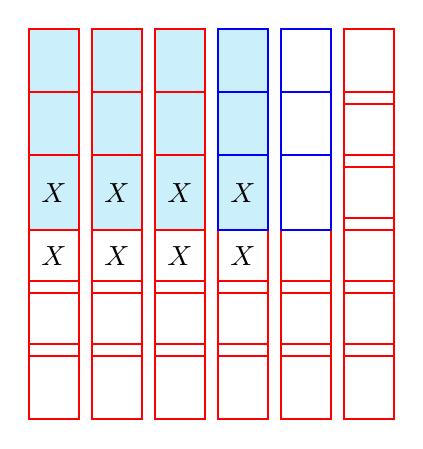
\begin{tikzpicture}[scale=0.8, >=stealth]
			% Vẽ các ô cơ bản (viền đỏ, nền trắng)
			\foreach \r in {1,...,6} {
				\foreach \c in {1,...,6} {
					\draw[thick, red] (\c-1, 6-\r) rectangle ++(0.8, 1.2);
				}
			}
			% Tô màu xanh nhạt (C)
			\foreach \r in {1,2,3} {
				\foreach \c in {1,2,3,4} {
					\draw[thick, red, fill=cyan!20] (\c-1, 6-\r) rectangle ++(0.8, 1.2);
				}
			}
			% Ghi đè viền xanh (B)
			\foreach \r in {1,2,3} {
				\foreach \c in {4,5} {
					\ifnum\c=4
					\draw[thick, blue, fill=cyan!20] (\c-1, 6-\r) rectangle ++(0.8, 1.2);
					\else
					\draw[thick, blue, fill=white] (\c-1, 6-\r) rectangle ++(0.8, 1.2);
					\fi
				}
			}
			% Thêm chữ X (X)
			\foreach \r in {3,4} {
				\foreach \c in {1,2,3,4} {
					\node at (\c-1+0.4, 6-\r+0.6) {$X$};
				}
			}
		\end{tikzpicture}
	\end{center}
	\par\shortans[0]{92}
	\loigiai{
		\textbf{Bước 1: Phân tích số lượng chậu cây và không gian mẫu}\\
		Có tổng cộng $36$ chậu cây, trong đó có $12$ chậu hoa hồng và $24$ chậu hoa cúc.\\
		Xếp ngẫu nhiên $36$ chậu cây vào $36$ ô trống, số phần tử của không gian mẫu (nếu phân biệt từng chậu cây) là
		$$n(\Omega) = 36!$$
		Tuy nhiên, vì ta chỉ quan tâm đến vị trí đặt các chậu "hoa hồng", ta có thể coi bài toán tương đương với việc chọn $12$ ô từ $36$ ô để đặt các chậu hoa hồng (các ô còn lại mặc nhiên đặt hoa cúc). Khi đó không gian mẫu thu gọn là $n(\Omega) = \mathrm{C}_{36}^{12}$.\\
		\textbf{Bước 2: Phân tích các tập hợp ô}\\
		Quan sát hình vẽ, ta chia các ô thành các tập hợp sau:
		\begin{itemize}
			\item Tập $C$ (tô màu): Gồm các ô thuộc $3$ hàng đầu, $4$ cột đầu. Số lượng $n(C) = 3 \times 4 = 12$ ô.
			\item Tập $X$ (chứa chữ X): Gồm các ô thuộc hàng $3$ và $4$, $4$ cột đầu. Số lượng $n(X) = 2 \times 4 = 8$ ô.
			\item Tập $B$ (viền xanh): Gồm các ô thuộc $3$ hàng đầu, cột $4$ và $5$. Số lượng $n(B) = 3 \times 2 = 6$ ô.
		\end{itemize}
		Để đếm chính xác, ta chia $36$ ô thành $7$ vùng rời nhau và đếm số ô mỗi vùng:
		\begin{itemize}
			\item Vùng 1: $C \cap X \cap B$ (tô màu, có X, viền xanh). Gồm đúng $1$ ô (hàng 3, cột 4). Gọi số ô là $n_1 = 1$.
			\item Vùng 2: $C \cap X \setminus B$ (tô màu, có X, viền đỏ). Gồm $3$ ô (hàng 3; cột 1, 2, 3). Gọi $n_2 = 3$.
			\item Vùng 3: $C \cap B \setminus X$ (tô màu, không X, viền xanh). Gồm $2$ ô (hàng 1, 2; cột 4). Gọi $n_3 = 2$.
			\item Vùng 4: $C \setminus (X \cup B)$ (tô màu, không X, viền đỏ). Gồm $6$ ô (hàng 1, 2; cột 1, 2, 3). Gọi $n_4 = 6$.
			\item Vùng 5: $X \setminus (C \cup B)$ (không màu, có X, viền đỏ). Gồm $4$ ô (hàng 4; cột 1, 2, 3, 4). Gọi $n_5 = 4$.
			\item Vùng 6: $B \setminus (C \cup X)$ (không màu, không X, viền xanh). Gồm $3$ ô (hàng 1, 2, 3; cột 5). Gọi $n_6 = 3$.
			\item Vùng 7 (phần còn lại): Gồm $36 - (1+3+2+6+4+3) = 17$ ô. Gọi $n_7 = 17$.
		\end{itemize}
		\textbf{Bước 3: Đếm số cách xếp thỏa mãn}\\
		Gọi $d_i$ là số chậu hoa hồng được xếp vào vùng $i$ ($i=1,\dots,6$). Theo giả thiết ta có hệ điều kiện
		$$\begin{cases}
			d_1 + d_2 + d_3 + d_4 = 4 & \text{(Tập C có 4 hoa hồng)} \\
			d_1 + d_2 + d_5 = 1 & \text{(Tập X có 1 hoa hồng)} \\
			d_1 + d_3 + d_6 = 1 & \text{(Tập B có 1 hoa hồng)}
		\end{cases}$$
		Từ phương trình thứ 2, ta xét $3$ trường hợp của bộ $(d_1, d_2, d_5)$:
		\begin{itemize}
			\item \textbf{TH1: $(d_1, d_2, d_5) = (1, 0, 0)$.}\\
			Thay vào hệ: $1 + d_3 + d_6 = 1 \Rightarrow d_3=0, d_6=0$. \\
			Và $1 + 0 + 0 + d_4 = 4 \Rightarrow d_4=3$. \\
			Vậy bộ $(d_1, d_2, d_3, d_4, d_5, d_6) = (1, 0, 0, 3, 0, 0)$. Số hoa hồng đã dùng là $4$, còn $8$ hoa hồng xếp vào vùng $7$.\\
			Số cách chọn ô: $W_1 = \mathrm{C}_1^1 \cdot \mathrm{C}_3^0 \cdot \mathrm{C}_2^0 \cdot \mathrm{C}_6^3 \cdot \mathrm{C}_4^0 \cdot \mathrm{C}_3^0 \cdot \mathrm{C}_{17}^8 = 1 \cdot 20 \cdot 24310 = 486\,200$.
			\item \textbf{TH2: $(d_1, d_2, d_5) = (0, 1, 0)$.}\\
			Thay vào hệ: $d_3 + d_6 = 1 \Rightarrow (d_3=1, d_6=0)$ hoặc $(d_3=0, d_6=1)$.
			\begin{itemize}
				\item Nếu $d_3=1, d_6=0 \Rightarrow d_4 = 4 - (0+1+1) = 2$. Bố trí: $(0, 1, 1, 2, 0, 0)$. Số hoa hồng dùng: $4$, vùng $7$ có $8$.\\
				$W_{2a} = \mathrm{C}_3^1 \cdot \mathrm{C}_2^1 \cdot \mathrm{C}_6^2 \cdot \mathrm{C}_{17}^8 = 3 \cdot 2 \cdot 15 \cdot 24310 = 2\,187\,900$.
				\item Nếu $d_3=0, d_6=1 \Rightarrow d_4 = 4 - (0+1+0) = 3$. Bố trí: $(0, 1, 0, 3, 0, 1)$. Số hoa hồng dùng: $5$, vùng $7$ có $7$.\\
				$W_{2b} = \mathrm{C}_3^1 \cdot \mathrm{C}_6^3 \cdot \mathrm{C}_3^1 \cdot \mathrm{C}_{17}^7 = 3 \cdot 20 \cdot 3 \cdot 19448 = 3\,500\,640$.
			\end{itemize}
			\item \textbf{TH3: $(d_1, d_2, d_5) = (0, 0, 1)$.}\\
			Thay vào hệ: $d_3 + d_6 = 1 \Rightarrow (d_3=1, d_6=0)$ hoặc $(d_3=0, d_6=1)$.
			\begin{itemize}
				\item Nếu $d_3=1, d_6=0 \Rightarrow d_4 = 4 - (0+0+1) = 3$. Bố trí: $(0, 0, 1, 3, 1, 0)$. Số hoa hồng dùng: $5$, vùng $7$ có $7$.\\
				$W_{3a} = \mathrm{C}_2^1 \cdot \mathrm{C}_6^3 \cdot \mathrm{C}_4^1 \cdot \mathrm{C}_{17}^7 = 2 \cdot 20 \cdot 4 \cdot 19448 = 3\,111\,680$.
				\item Nếu $d_3=0, d_6=1 \Rightarrow d_4 = 4 - (0+0+0) = 4$. Bố trí: $(0, 0, 0, 4, 1, 1)$. Số hoa hồng dùng: $6$, vùng $7$ có $6$.\\
				$W_{3b} = \mathrm{C}_6^4 \cdot \mathrm{C}_4^1 \cdot \mathrm{C}_3^1 \cdot \mathrm{C}_{17}^6 = 15 \cdot 4 \cdot 3 \cdot 12376 = 2\,227\,680$.
			\end{itemize}
		\end{itemize}
		Tổng số cách chọn vị trí cho $12$ chậu hoa hồng là
		$$n(A) = W_1 + W_{2a} + W_{2b} + W_{3a} + W_{3b} = 11\,514\,100 \text{ (cách)}.$$
		\textbf{Bước 4: Tính xác suất}\\
		Xác suất thỏa mãn yêu cầu bài toán là
		$$p = \dfrac{n(A)}{n(\Omega)} = \dfrac{11\,514\,100}{1\,251\,677\,700} \approx 0,0091989$$
		Vậy $10000p = 91,989$. Làm tròn kết quả đến hàng đơn vị, ta được $\boxed{92}$.
	}
\end{ex}